\documentclass[../report.tex]{subfiles}

\begin{document}

%%% \subsection{Crowdsourcing}

% ad hoc
A survey on crowdsourcing \cite{Oerting2019Survey} found that several medical image analysis research papers lack description of annotation task design choices. It concludes that withholding information on the motivating factors and considerations behind designing the characteristics of annotation tasks, causes studies to be less accurately reproducible. This in turn makes crowdsourcing less approachable to resaerchers who do not have experience with conducting crowdsourced annotation. The characteristics of crowdsourcing tasks identified in the survey include \textit{platform choice}, \textit{number of annotators}, and \textit{how the task is explained to annotators}. This survey acts as a literature review of studies that apply crowdsourcing in medical image analysis, and it highlights the need for increased guidance in conducting crowdsourcing, through better documentation of experiments. \\

% mturk
Researchers in medical image analysis are typically not trained in design or development, and thus leverage existing frameworks. A popular option is Amazon's Mechanical Turk (MTurk) \cite{mturk}, which connects researchers with workers, while handling infrastructure and scalability. It also provides pre-built annotation tasks, which means researchers only have to feed their training data to the platform. For these reasons, it is an obvious choice for many researchers, but it also lessens the burden of considering the aforementioned characters of crowdsourcing. Researchers do not have to describe motivating factors, as MTurk workers are financially incentivized to complete the given annotation task.

%%% \subsection{Interaction Design}

There are numerous examples of research applying crowdsourcing in medical image analysis. In the following section, examples of research approaches in crowdsourcing are presented. \\

% herrera et al.
Herrera et al. \cite{herrera2014crowd} took another approach to crowdsourcing, arguably one with less of a 'crowd'. They produced algorithmic classifications of their dataset, and then leveraged the Crowdflower platform to connect with a small group of eight medical imaging experts. These crowdsourced workers were tasked with verifying the algorithmic classifications. Each image in their dataset contained at least two crowdsourced annotations, and a third for images with opposing annotations.

These researchers found that the expert workers lacked some knowledge to complete their tasks, but that crowdsourcing was especially useful for annotating low-resolution imagery. They also conclude that while they chose a small pool of workers in the medical imaging domain, they could have taken the opposing approach by applying stricter quality control.

% Crowdsourcing for Reference Correspondence Generation in Endoscopic Images
Maier-Hein et al. \cite{maier2014endoscopic} leveraged MTurk in asessing the quality of crowdsourced annotations for medical endoscopic images. They supplied MTurk with their own user interface written in HTML5/JavaScript, but they do not indicate why this choice was made or whether any considerations were had about the design of this interface.  They find a median annotation error of 2 px, which is twice that of medical experts, but through cluster analysis of multiple annotations per image, they reduce errors so that they are comparable to expert classifications.

In their discussion, they identify annotation tasks as consisting of multiple tasks that in combination result in a classification. Their point is that while some tasks may require expert knowledge or experience, the task they crowdsourced appears to have produced comparable classifications while leveraging non-experts.\\

% braindr.us
Braindr \cite{Braindr} is an app for quality control of images from the Healthy Brain Network \cite{Alexander2017HealthyBrain}. Rather than conducting crowdsourcing through a platform, its annotation tasks are custom and do not offer financial incentives. This meant the creators had to find other motivating factors, and they chose to gameify the process through a point-system and leaderboard. \\

\begin{figure}[h]
\centering
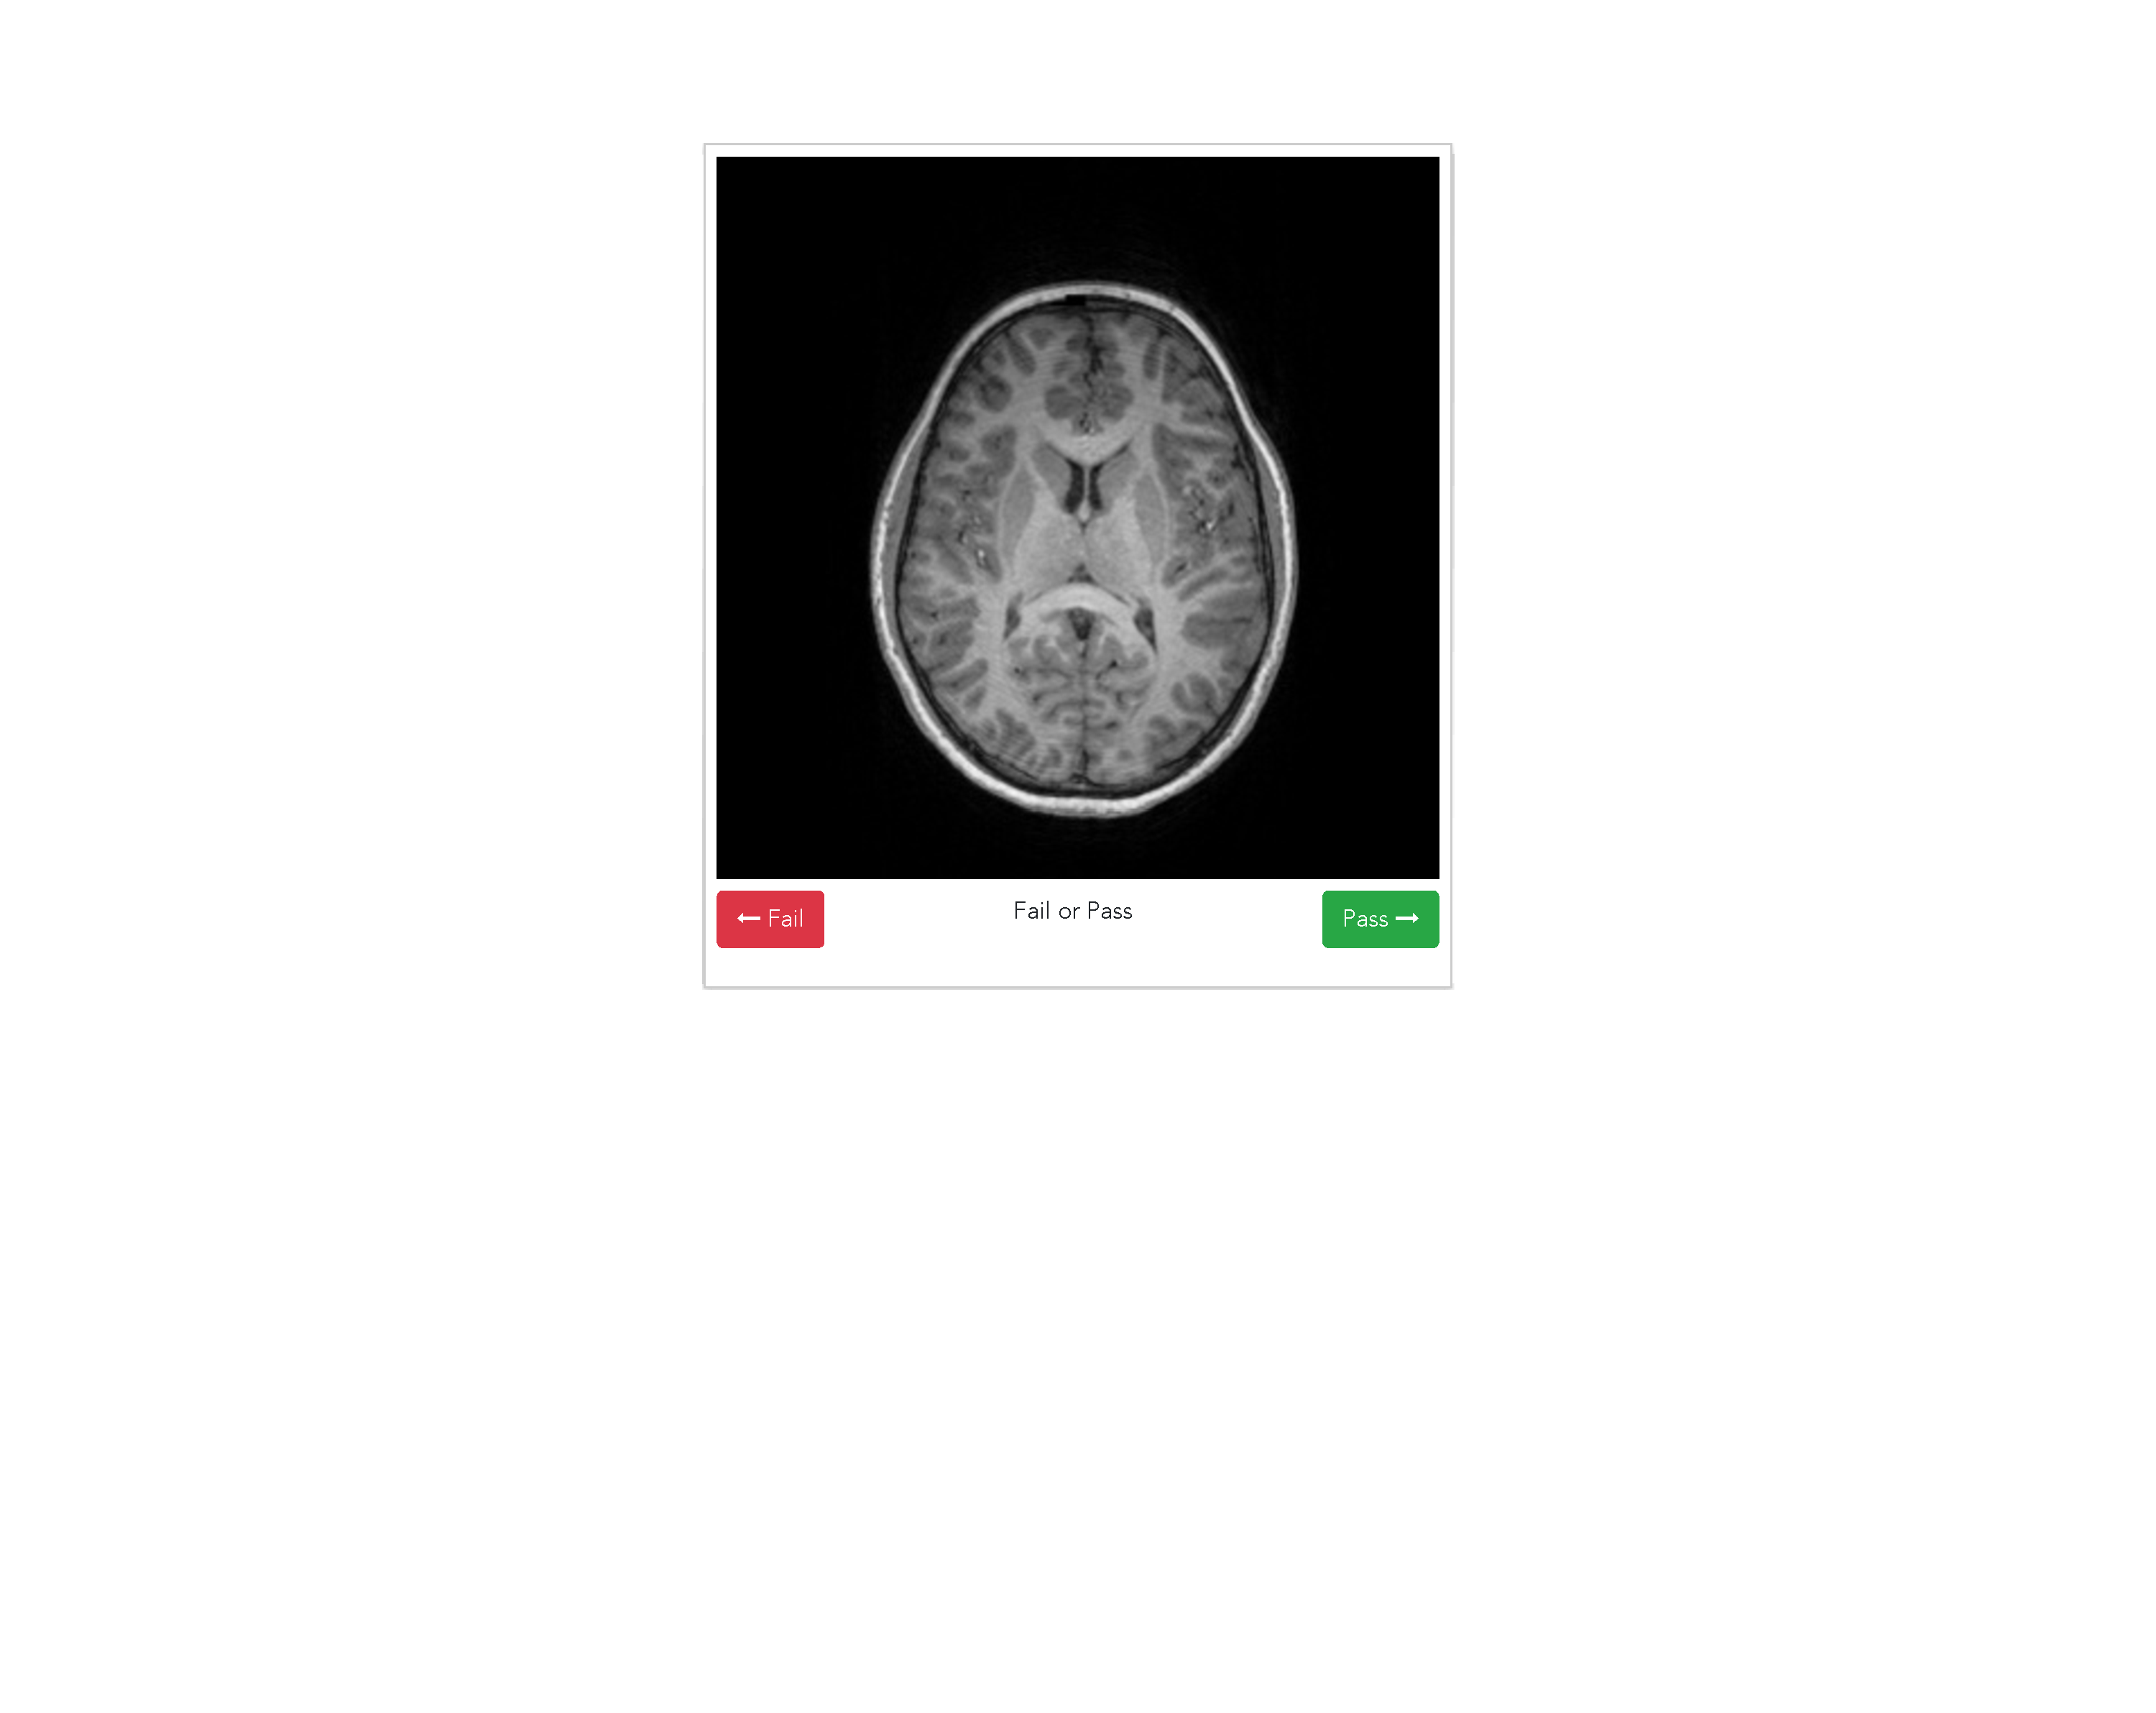
\includegraphics[width=0.8\linewidth]{braindr.pdf}
\caption{Example of a discrete annotation task in crowdsourced medical imaging. \cite{Braindr}}
\label{figure:braindr}
\end{figure}

In their evaluation, they chose to filter out image annotations that had not been repeated at least 5 times. They conclude based on the produced annotations that while some images fit well into the discrete classification of fail or pass, there are also images that do not. This raises questions about whether their task design is extensive enough, in that it evidently may not cover all scenarios during annotation. If an image is perceived as neither passing nor failing, then annotators are only given the choice to provide incorrect annotations, due to the lack of a "neither" or "unsure" option. \\

% interaction attributes
The quality difference between a set of interactions can be assessed by establishing their interaction profile. In Human-Computer Interaction (HCI) research exists an Interaction Vocabulary consisting of attributes that describe interfacing between humans and technology, as well as the relationship between the expectations of designers and the reality users experience \cite{Lenz2013Attributes}. \\

\begin{table}[h]
\centering
\begin{tabular}{c c}
\hline
\textbf{Minimum} & \textbf{Maximum} \\ [0.5ex]
\hline
slow & fast \\
stepwise & fluent \\
instant & delayed \\
uniform & diverging \\
constant & inconstant \\
mediated & direct \\
spatial separation & spatial proximity \\
approximate & precise \\
gentle & powerful \\
incidental & targeted \\
apparent & covered \\ [1ex] 
\hline
\end{tabular}
\caption{Interaction attributes}
\label{table:attributes}
\end{table}

The authors conclude that interactions should be judged by whether the designer's intent matches the user's perception, meaning that no interaction attribute should be viewed as greater or more desirable than others. Instead, attributes should be viewed as appropriate relative to whether they produce a perception that matches the intent. \\

Based on their findings, it is hypothesised that the annotation task best perceived as it was intended must have the best fit of interaction attributes. In the context of annotation, the attributes \textit{stepwise, instant, uniform, direct, spatial proximity, and precise} (table \ref{table:attributes}) are expected to reflect an ideal experience.

\end{document}